% !TeX root = ../main.tex
\chapter{Literature Review}
\label{chap:literature}


\section{Related Work}
\label{sec:related-work}
\begingroup
\setlength{\emergencystretch}{2em}

\subsection{FIU 2024: Pedro Chaviano's Vacuum Crawler}
\label{sec:previous-fiu-crawlers}
\label{sec:fiu-2024-crawler}
Pedro Chaviano's 2024 internship work investigated a remotely operated vacuum crawler for cleaning the DST annulus. The prototype combined a mobile platform and pneumatic debris collection, establishing a starting point for subsequent FIU development \citep{chaviano2025Crawler}. Figure~\ref{fig:pedro-crawler} shows this prototype.

Chaviano's prototype used a three-dimensionally printed plastic chassis, four-wheel differential drive, and a small EXAIR Venturi vacuum module approximately 1~in in diameter. It used analog control with a Raspberry Pi Pico and did not use camera feedback \citep{chaviano2025Crawler}. Chaviano conducted debris-removal experiments; the reported vacuuming efficiency from 22\% to 95\%. The prototype used a vacuum line rather than an onboard collection bag, requiring debris to travel approximately 40ft to the collection point. That long conveying path may have contributed to the low measured efficiency, although the available report does not establish it as the cause. The prototype was not robust, and its vacuuming properties were not characterized sufficiently to establish reliable performance. Remaining work included a metal chassis, further mobility testing with its added mass, and additional cleaning and sensing functions.

\begin{figure}[H]
\centering
\thesisimage{Vacuum_Pedro.png}
\caption[FIU 2024 vacuum crawler: Pedro Chaviano]{FIU 2024 vacuum crawler developed by Pedro Chaviano. Project image supplied by the author.}
\label{fig:pedro-crawler}
\end{figure}

This version established the feasibility of combining remote mobility with pneumatic cleaning. Its prototype construction and configuration-dependent results motivated continued development of the chassis, collection arrangement, and operating controls. These earlier contributions form part of the project's inherited foundation.

\subsection{FIU 2025: Ronald Verde's Vacuum Crawler}
\label{sec:fiu-2025-crawler}
Ronald Verde continued the crawler's development during 2025. His version used an aluminum chassis, treaded aluminum wheels, and an onboard collection bag, with both pneumatic modules located on the crawler \citep{verde2025Crawler}. These changes provided a metal platform with the collection components integrated onto the vehicle, shown in Figure~\ref{fig:ronald-crawler}.

\begin{figure}[H]
\centering
\thesisimage{Vacuum_Ronald.png}
\caption[FIU 2025 vacuum crawler: Ronald Verde]{FIU 2025 vacuum crawler developed by Ronald Verde. Project image supplied by the author.}
\label{fig:ronald-crawler}
\end{figure}

Although the chassis was made from aluminum, the center of gravity was shifted forward relative to the wheel placement. As observed by the author, the crawler consequently tilted backward during operation, preventing the pickup inlet from maintaining the position needed for vacuuming. The inherited crawler also could not turn within the annulus or traverse the required obstacles. The aluminum construction therefore did not resolve the practical cleaning and mobility requirements of the project. These limitations motivate the present work on debris collection, maneuverability, and obstacle traversal with the complete crawler and its attached hose.


% Attribution confirmed by the author on October 11, 2026: despite the
% 2025 report's ROS 2 claims, the inherited crawler did not implement ROS 2.
% Do not cite that report as evidence of an earlier ROS 2 implementation.

\subsection{Rolls-Royce Annulus Cleaning System}
\label{sec:rolls-royce-cleaner}
Rolls-Royce developed a robotic cleaning system for debris that obstructed inspection and level monitoring in the Hanford tank annulus. The technology roadmap describes mechanically relocating debris or removing it through containers. Following factory testing, the system was demonstrated to Hanford personnel in Richland in 2019, and operators received training \citep{hanford2022AnnulusCleaner}. Figure~\ref{fig:rolls-royce-cleaner} shows the reported mockup.

\begin{figure}[H]
\centering
\thesisimage[trim=111.6bp 80.4bp 103.8bp 312.6bp,clip]{references/Rolls Royce Cleaner.png}
\caption[Rolls-Royce annulus floor cleaner mockup]{Annulus floor cleaner mockup reported for the Rolls-Royce system \citep{hanford2022AnnulusCleaner}.}
\label{fig:rolls-royce-cleaner}
\end{figure}

The roadmap records successful factory acceptance testing and lists the cleaning activity as complete and retired \citep{hanford2022AnnulusCleaner}. The available roadmap does not report conduit-crossing performance or explain why the activity was retired. The pictured wheel geometry appears to offer limited ability to cross raised conduits, but this visual observation is not a demonstrated performance result. The system's reported configuration is more consistent with a floor-cleaning platform than a vacuum-based debris-transport system; this distinction is relevant because the present project requires debris to be conveyed into a collection system.

The system demonstrates prior remote annulus-cleaning development. Its retired status and the limits of what the available documentation establishes provide context for the remaining project requirements: debris collection and transport, access across the required obstacles, and retrieval.

\subsection{Summary of Existing Annulus Cleaning Technologies}
\label{sec:annulus-cleaning-technology-summary}
The systems reviewed for this application comprise two FIU vacuum-crawler prototypes and the Rolls-Royce annulus floor-cleaning system. They represent different approaches: pneumatic debris conveyance through a vacuum line, an aluminum crawler with an onboard collection bag, and a remotely operated floor-cleaning platform. The FIU prototypes provide project-specific evidence of attempted vacuum collection, while the Rolls-Royce roadmap documents factory acceptance testing, a 2019 demonstration, and eventual retirement of the activity \citep{chaviano2025Crawler,verde2025Crawler,hanford2022AnnulusCleaner}.

Each documented system has limitations against the present project's combined requirements. Chaviano's prototype had limited characterization and robustness, and its long vacuum line may have reduced recovery. Verde's crawler did not maintain pickup orientation and could not turn or traverse the required obstacles, based on the author's observations of the inherited system. The Rolls-Royce source does not report vacuum-based debris transport or conduit-crossing results; its pictured geometry suggests possible access limitations, but this requires operational evidence. The author reports that all three systems have since been decommissioned. Their documented limitations mean they do not provide a currently available, demonstrated solution to this project's requirements; the available records do not establish a common reason for decommissioning.

The research need is therefore an integrated crawler that can be deployed through the riser, collect and retain the target debris, maneuver in the annulus, cross the specified protective pipes, and be retrieved with its hose and controls attached. The reviewed technologies establish relevant starting points, but do not demonstrate all of these functions together. Figure-based judgments about the Rolls-Royce system remain hypotheses until supported by test or project records.
\par
\endgroup

\section{Vacuum Generation and Debris Collection Technologies}
\label{sec:vacuum-technologies}
\begingroup
\setlength{\emergencystretch}{2em}

The annulus cleaner requires a source of suction and a way to retain the recovered debris for later disposal, or to convey it to a disposal point. This section reviews pneumatic conveyors, electric vacuum motors, and side-channel blowers, focusing on how their airflow arrangements produce suction and transport air through the collection path.

\subsection{Compressed-Air Venturi Vacuum Systems}
\label{sec:venturi-vacuums}
Pneumatic vacuum generators use compressed air to produce suction without a rotating impeller. In a Venturi ejector, an accelerated air stream draws air through a suction connection, and both streams leave through the exhaust. Compact ejectors are widely used in vacuum handling, including gripping airtight workpieces \citep{schmalzVacuumEjectors}. For debris collection, however, the device must also provide a passage suitable for the material being transported; a suction-gripping ejector is not automatically a solids conveyor.

The EXAIR Line Vac is an example of an air-operated conveyor relevant to this distinction. Directed compressed-air jets create suction at its intake and accelerate material through an open bore into the discharge hose. The device has no moving parts, and its conveying rate can be adjusted through the supply-pressure regulator \citep{exairLineVacCatalog}. This arrangement is relevant to a compact crawler because the conveying module can be located near the pickup point without an onboard vacuum motor.

\begin{figure}[H]
\centering
\resizebox{0.9\textwidth}{!}{%
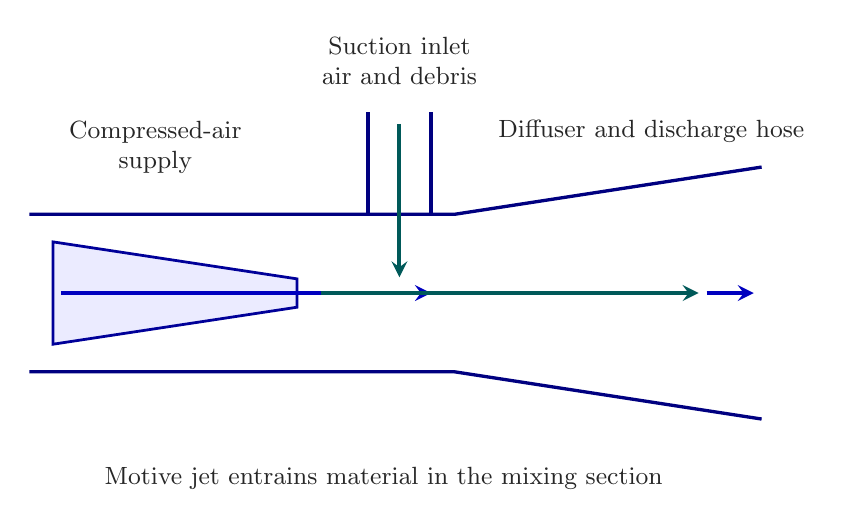
\begin{tikzpicture}[
  >=stealth,
  air/.style={->,line width=1.5pt,draw=blue!75!black},
  mix/.style={->,line width=1.5pt,draw=teal!70!black},
  shell/.style={draw=blue!50!black,line width=1.2pt},
  label/.style={font=\small,align=center,text=black!85}
]
% Conveying tube and expanding discharge diffuser.
\draw[shell] (0.4,0.8) -- (5.8,0.8) -- (9.7,0.2);
\draw[shell] (0.4,2.8) -- (5.8,2.8) -- (9.7,3.4);
% Compressed-air nozzle and its motive jet.
\path[draw=blue!60!black,fill=blue!8,line width=1pt]
  (0.7,1.15) -- (3.8,1.62) -- (3.8,1.98) -- (0.7,2.45) -- cycle;
\draw[air] (0.8,1.8) -- (5.5,1.8);
% Suction branch joins the low-pressure mixing region.
\draw[shell] (4.7,2.8) -- (4.7,4.1);
\draw[shell] (5.5,2.8) -- (5.5,4.1);
\draw[mix] (5.1,3.95) -- (5.1,2.0);
\draw[mix] (4.1,1.8) -- (8.9,1.8);
\draw[air] (9.0,1.8) -- (9.6,1.8);
\node[label] at (2.0,3.65) {Compressed-air\\supply};
\node[label] at (5.1,4.75) {Suction inlet\\air and debris};
\node[label] at (4.9,-0.55) {Motive jet entrains material in the mixing section};
\node[label] at (8.3,3.85) {Diffuser and discharge hose};
\end{tikzpicture}%
}
\caption[Venturi conveyor airflow principle]{Conceptual Venturi-conveyor airflow: compressed air accelerates through a nozzle, draws material through the suction inlet, and carries the combined stream toward the discharge. The schematic illustrates the operating principle described for the EXAIR Line Vac \citep{exairLineVacCatalog}.}
\label{fig:EXAIR Compressed Air}
\end{figure}

Its main limitations concern the air supply and the downstream collection path. EXAIR identifies conveying distance, vertical lift, bends, material characteristics, and input pressure as factors requiring application-specific testing. Powder collection also requires separation of the material from the discharged air \citep{exairLineVacFAQ}. The manufacturer cautions against opposing discharge pressure and undersized outlet piping \citep{evans2013LineVacBackPressure}. For this project, the receiver and filter must therefore accommodate the combined conveying and compressed-air flow without excessive restriction. A compact module alone does not establish adequate pickup, acceptable air consumption, or reliable operation as the collector loads with debris.

\subsection{Electric Motor-Driven Vacuum Systems}
\label{sec:electric-vacuums}
An electric vacuum motor rotates an impeller or fan to move air from the inlet toward the exhaust. The moving air lowers pressure at the inlet, drawing air and entrained debris through the pickup nozzle and hose. In a through-flow motor, the working air also passes through and cools the motor; in a bypass motor, a separate airflow cools the motor while the working stream follows its own path through the vacuum unit \citep{garantola2023UniversalBlowers}. In either arrangement, the collector and filter sit in the working-air path and must separate debris without restricting the flow excessively.

Fan geometry and stage count determine the balance between airflow and pressure rise: single-stage designs generally favor airflow at lower pressure differences, while additional stages can increase pressure capability \citep{garantola2023UniversalBlowers}. Airflow carries debris through the line, while pressure must overcome losses at the pickup, hose, collector, and filter. For the crawler, an electric source could remain outside the deployment envelope, but its performance depends on the complete connected path. Testing should therefore measure airflow and debris recovery with the intended nozzle, hose, collector, and filter; motor rating alone does not establish pickup or transport performance.

\begin{figure}[H]
\centering
\resizebox{0.94\textwidth}{!}{%
\begin{tikzpicture}[
  >=stealth,
  component/.style={draw=blue!55!black,fill=blue!4,rounded corners=3pt,
    minimum height=13mm,align=center,font=\small,inner sep=5pt},
  flow/.style={->,line width=1.1pt,draw=teal!70!black},
  note/.style={font=\footnotesize,align=center,text=black!75}
]
\node[component] (pickup) {Pickup\\inlet};
\node[component,right=7mm of pickup] (hose) {Hose\\airflow};
\node[component,right=7mm of hose] (collector) {Collector\\and filter};
\node[component,right=7mm of collector] (motor) {Impeller\\and motor};
\node[component,right=7mm of motor] (exhaust) {Exhaust};
\draw[flow] (pickup) -- (hose);
\draw[flow] (hose) -- (collector);
\draw[flow] (collector) -- (motor);
\draw[flow] (motor) -- (exhaust);
\node[note,below=9mm of collector,text width=115mm] {Working airflow carries debris through the hose; the collector and filter retain solids before air reaches the motor. In a through-flow design, this filtered air also provides motor cooling.};
\end{tikzpicture}%
}
\caption[Airflow path through an electric vacuum motor]{Conceptual airflow path through a through-flow electric vacuum system. The collector and filter remove debris before air reaches the motor.}
\label{fig:electric-vacuum-airflow}
\end{figure}

\subsection{Regenerative or Side-Channel Blower Systems}
\label{sec:side-channel-blowers}
A regenerative, or side-channel, blower also uses an electric motor and rotating impeller, but moves air through a ring-shaped side channel. As the impeller turns, it repeatedly transfers energy to the gas circulating through the channel, producing a pressure difference between the inlet and outlet. Repeated energy transfer allows the blower to sustain suction or pressure without contact between the impeller and housing \citep{buschSideChannelTechnology}. Unlike the vacuum-motor arrangements above, the gas remains in the blower's channel as it gains energy; the connected hose, collector, and filter still determine the airflow available at the pickup point.

The blower moves air rather than separating debris, so a collector and filter must retain solids upstream and protect its inlet. Resistance from the hose, loaded filter, or blockage can reduce airflow and affect cooling; Busch consequently requires suitable dust filtration, adequate cooling and minimum gas flow, and pressure relief where the inlet may be closed \citep{buschSamosSIManual}. For this project, its suitability as an external source depends on airflow through the actual hose, separator, and filter. Continuous-duty capability alone does not establish debris-conveying performance.

\begin{figure}[H]
\centering
\resizebox{0.94\textwidth}{!}{%
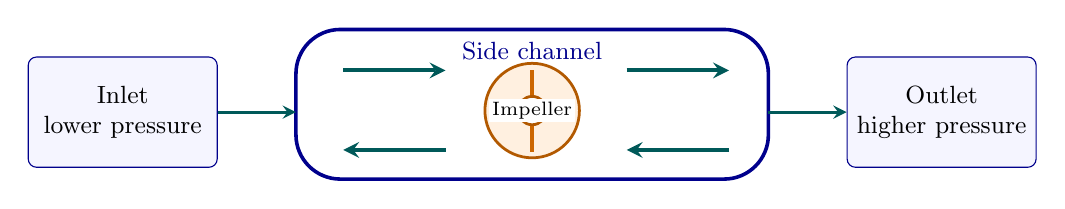
\begin{tikzpicture}[
  >=stealth,
  port/.style={draw=blue!55!black,fill=blue!4,rounded corners=3pt,
    minimum width=24mm,minimum height=14mm,align=center,font=\small},
  flow/.style={->,line width=1.1pt,draw=teal!70!black},
  channel/.style={draw=blue!55!black,line width=1.3pt,rounded corners=16pt},
  note/.style={font=\footnotesize,align=center,text=black!75}
]
\node[port] (inlet) at (0,1.1) {Inlet\\lower pressure};
\node[port] (outlet) at (10.4,1.1) {Outlet\\higher pressure};
\draw[channel] (2.2,0.25) rectangle (8.2,2.15);
\node[font=\small,text=blue!55!black] at (5.2,1.88) {Side channel};
\draw[fill=orange!12,draw=orange!70!black,line width=1pt] (5.2,1.12) circle (0.60);
\draw[fill=white,draw=orange!70!black,line width=1pt] (5.2,1.12) circle (0.18);
\foreach \a in {0,90,180,270} {
  \draw[draw=orange!80!black,line width=1.4pt] (5.2,1.12) ++(\a:0.20) -- ++(\a:0.32);
}
\node[font=\scriptsize,fill=white,inner sep=1pt] at (5.2,1.12) {Impeller};
\draw[flow] (inlet.east) -- (2.2,1.1);
\draw[flow] (8.2,1.1) -- (outlet.west);
\draw[flow,line width=1.5pt] (2.8,1.63) -- (4.1,1.63);
\draw[flow,line width=1.5pt] (6.4,1.63) -- (7.7,1.63);
\draw[flow,line width=1.5pt] (7.7,0.62) -- (6.4,0.62);
\draw[flow,line width=1.5pt] (4.1,0.62) -- (2.8,0.62);
\end{tikzpicture}%
}
\caption[Side-channel blower airflow principle]{Conceptual side-channel blower principle. The impeller transfers energy to gas circulating through the channel, creating a pressure difference between inlet and outlet.}
\label{fig:side-channel-airflow}
\end{figure}

\subsection{Suitability for Annulus Debris Removal}
\label{sec:vacuum-annulus-suitability}
The reviewed technologies differ in how they create suction and move debris through the collection path. For the initial vacuum tests in this project, a compressed-air Venturi conveyor is selected as the primary candidate. This is a test-selection decision based on mechanical and integration considerations; it does not establish that the Venturi system will outperform an electric vacuum motor or side-channel blower.

The Venturi arrangement has a simple conveying module with no moving parts, and its open bore is designed to carry material in the induced airflow \citep{exairLineVacCatalog}. Compared with an electric motor-driven unit, it avoids placing a rotating motor and impeller on the crawler and does not require motor cooling or electrical drive hardware at the pickup point. The compressed-air generator can be located remotely while the compact conveyor remains near the intake, which supports a simpler crawler package and keeps motor servicing outside the deployment envelope. The prior FIU crawler prototypes also used pneumatic conveying modules, so testing this approach first provides continuity with the inherited project architecture \citep{chaviano2025Crawler,verde2025Crawler}. These are reasons to prioritize the configuration for evaluation, not evidence of a measured mass, reliability, or recovery advantage.

The approach has corresponding costs and open questions. It depends on a suitable compressed-air supply and its pressure and flow must remain adequate through the intended service line. The combined motive air and conveyed material also require a receiver and filter that separate and retain the debris without excessive discharge resistance. Hose length, bends, lift, debris properties, and downstream restriction can affect conveying and must be represented in testing \citep{exairLineVacFAQ,evans2013LineVacBackPressure}. The open bore and absence of moving parts do not by themselves prove that blockages will be less frequent or that recovery will meet the project target.

The test configuration should therefore use the intended pickup, hose route, receiver, and filter, and record recovery, conveying time, blockage, and compressed-air demand under controlled conditions. Results will determine whether the Venturi arrangement remains suitable for the integrated crawler. Electric motor-driven vacuum and side-channel architectures remain valid alternatives if the measured pneumatic performance or utility demand is inadequate. Chapter~\ref{chap:design} will document the implemented configuration, while Chapter~\ref{chap:methods} will describe the comparative tests and operating conditions.
\par
\endgroup

\section{Crawler Mechanical Configurations and Mobility}
\label{sec:crawler-mechanical-configurations}
\begingroup
\setlength{\emergencystretch}{2em}
\clubpenalty=10000
\widowpenalty=10000

% Start this section's introduction at 2.30; the comparisons remain 2.31--2.33.
\setcounter{subsection}{-1}
\subsection{Introduction}
\label{sec:mechanical-configurations-introduction}
The crawler must carry the vacuum equipment and position the pickup while moving through the annulus. The relevant mechanical choices concern the chassis configuration, the locomotion system, and the compliance available to accommodate changes in the floor profile. This section reviews these choices in relation to equipment support, maneuverability, and passage over protective pipes.

\subsection{Chassis Configurations}
\label{sec:chassis-configurations}
Chassis articulation and suspension describe related but distinct features. Articulation allows connected frame sections or wheel-support assemblies to rotate relative to one another. Suspension allows wheel movement relative to the main body to accommodate terrain and loading. The two can overlap: a jointed bogie can serve as a suspension mechanism without springs, while a rigid main body can carry independently suspended wheels. Here, a rigid chassis refers to a frame with fixed wheel mounting positions and no suspension travel; tire deformation is considered separately.

A rigid chassis provides fixed attachment locations for the vacuum equipment and pickup, without joints between frame sections or moving wheel supports. For this project, that arrangement simplifies equipment mounting and keeps the relative positions of the components fixed. Its limitation is ground accommodation. When the four supporting points lie at unequal elevations, the frame cannot adjust individual wheel positions, so wheel loading can become uneven and a wheel may lose contact. Bouton and Gao's analysis contrasts rigid four-point support with a passive bogie, which permits unequal wheel elevations while approximately equalizing the loads on its two wheels \citep{bouton2023Marcel}.

An articulated chassis can accommodate changes in terrain through its joints, although the available motion depends on the joint axes. A steering joint alone does not provide vertical wheel travel. In the MARCEL rover, a central steering joint and a rear bogie provide distinct motions; active bogie torque also redistributes wheel loading. The central joint occupies equipment space, while bogie placement affects both payload accommodation and ground clearance \citep{bouton2023Marcel}. For a vacuum crawler, equipment and hoses spanning moving sections would consequently need to accommodate that motion.

A rigid main body with suspension offers another arrangement: the equipment remains on a common frame while the wheel supports move. Passive suspension accommodates terrain through its mechanical response, whereas active suspension adds controlled adjustment of wheel position or loading. These mechanisms can improve wheel contact, but add joints and supporting components; active arrangements also require actuation and control. The suspension configurations reviewed by Bouton and Gao illustrate this tradeoff between terrain adaptation and mechanical complexity \citep{bouton2023Marcel}.

Neither articulation nor suspension alone establishes adequate clearance or stability. Otsu et al. show that clearance estimates for articulated rovers depend on the body pose produced by terrain contact \citep{otsu2020Clearance}. Papadopoulos and Rey likewise relate tipover stability to the support contacts, center of mass, and external forces and moments \citep{papadopoulos1996Stability}. Applied to the crawler, these findings favor low equipment placement within the supported footprint while preserving space beneath the pickup and frame. Hose forces must also be considered because their direction and attachment location can produce a tipping moment.

A rigid chassis is therefore a reasonable practical choice for supporting the vacuum equipment with a simple mounting arrangement. It avoids the additional mechanisms and motion allowances associated with articulation or suspension. This choice accepts a limited ability to accommodate uneven ground: wheel contact, underside clearance, and stability must still be assessed during obstacle crossing.

\subsection{Wheeled versus Tracked Locomotion}
\label{sec:wheeled-tracked-locomotion}
Wheels and tracks offer different compromises between traction and mechanical complexity. Wheels provide separate ground contacts, while tracks distribute contact along a continuous belt. Mandow et al. identify generally better traction from tracked locomotion, together with greater mechanical complexity \citep{mandow2007Kinematics}. For the annulus crawler, wheels provide a practical arrangement around the equipment-carrying frame. A tracked alternative would require space for the track path and its supporting and driving components. The traction advantage must therefore be weighed against integration requirements; neither arrangement establishes pipe-crossing capability without considering its geometry and contact conditions.

The selected four-wheel arrangement uses left-right differential drive with fixed wheel axes. Differences between the speeds on the two sides turn the crawler through skid steering, which requires lateral wheel slip. Opposite drive directions permit turning within a small footprint without separate steering hardware, although actual motion depends on ground contact \citep{mandow2007Kinematics}. This is relevant to maneuvering within the annulus, where turning space is restricted. Skid steering also introduces resistance during turns: Shamah's same-rover comparison on natural terrain found higher power and wheel torque than with explicit wheel steering, particularly in tight turns \citep{shamah1999SkidSteering}.

Compliant tires provide local deformation at the contact without introducing chassis suspension. Their selection must account for both forward traction and lateral sliding during turns. Mandow et al.'s tests with solid-rubber and pneumatic tires showed that tire construction and inflation affected skid-steering behavior; the tested wheel sets also differed in diameter, so the results do not establish a universally preferable tire material \citep{mandow2007Kinematics}. For this crawler, compliance is a means of accommodating local contact geometry, rather than a guarantee of improved traction under every condition.

\label{sec:obstacle-traversal-review}
Wheel diameter, tire deformation, and available drive torque also influence obstacle traversal. Wilhelm et al. relate step climbing to obstacle height relative to wheel radius and show that a larger radius does not necessarily reduce the required axle torque. In tests with a driven, foam-filled tire, deformation stored and released elastic energy, affecting climbing under an abrupt torque input \citep{wilhelm2007StepClimbing}. These findings support considering wheel size and compliance together. Larger wheels also consume deployment space, while tire deformation changes the loaded wheel geometry; both must be considered when selecting clearance for the crawler.

The rigid four-wheel platform retains limitations that compliant tires cannot fully overcome. Tire deformation provides only local accommodation and cannot independently reposition a wheel as a suspension can. Uneven loading or loss of contact can therefore reduce the traction available for climbing. The pickup and underside must also clear the obstacle as it passes between the axles; front-wheel ascent alone does not establish successful traversal. In addition, the sharp step modeled by Wilhelm et al. differs from a protective pipe: the pipe presents a curved contact surface and requires descent after the crest \citep{wilhelm2007StepClimbing}. Published step-climbing results consequently inform wheel selection but do not establish this crawler's pipe-crossing limit.

\subsection{Summary and Design Implications}
\label{sec:mechanical-design-implications}
The reviewed findings support a rigid chassis with four-wheel differential/skid steering and compliant tires as a practical configuration for carrying the vacuum equipment and maneuvering through the annulus. The arrangement combines fixed equipment mounting with steering through the drive wheels and local compliance at the tires. Its main limitations remain uneven wheel loading, turning resistance, and clearance and stability during pipe crossing. Chapter~\ref{chap:design} presents the selected dimensions, construction, and implementation; Chapter~\ref{chap:methods} describes evaluation with the complete crawler and its attached hose.
\par
\endgroup

\section{Research Gap and Implications for This Project}
\label{sec:research-gap}
The reviewed annulus-cleaning systems provide a starting point for this project, but do not demonstrate all of its cleaning and access requirements together. Chaviano's prototype combined remote mobility with pneumatic debris conveyance, while Verde's later version introduced the inherited aluminum platform and onboard collection arrangement \citep{chaviano2025Crawler,verde2025Crawler}. As discussed in Section~\ref{sec:related-work}, the author observed inadequate pickup orientation, restricted turning, and unsuccessful obstacle traversal in the inherited crawler. The Rolls-Royce system provides evidence of remote annulus-cleaning development, but its available record does not establish vacuum-based debris transport or protective-pipe crossing \citep{hanford2022AnnulusCleaner}. These limitations define the project need without implying that the earlier systems lacked value or shared the same reason for retirement.

The vacuum review identifies a compressed-air Venturi conveyor as the initial candidate for evaluation because of its simple conveying module, open material passage, and compatibility with the inherited pneumatic arrangement. Its suitability still depends on the complete pickup and collection path. Conveying distance, bends, supply conditions, and downstream resistance affect material transport \citep{exairLineVacFAQ,evans2013LineVacBackPressure}. The remaining question is therefore whether the selected arrangement can recover and retain the target debris with acceptable compressed-air demand under the intended operating conditions. Electric vacuum motors and side-channel blowers remain alternatives if the pneumatic arrangement proves inadequate; the review does not establish a measured performance ranking among them.

The mechanical review supports a rigid chassis with four-wheel differential/skid steering and compliant tires as a practical configuration for mounting the vacuum equipment and maneuvering within the annulus. It also identifies the limits that must be addressed: uneven wheel loading, resistance during skid steering, and clearance and stability as the crawler crosses protective pipes. Articulation and suspension can provide additional terrain accommodation, while tire compliance acts locally at the wheel contact \citep{bouton2023Marcel,wilhelm2007StepClimbing,mandow2007Kinematics}. The reviewed findings explain these tradeoffs but do not establish the traversal capability of the selected rigid platform with its equipment and hose attached.

The gap addressed by this thesis is the characterization of vacuum performance and compressed-air use, together with the integration and evaluation of the collection system on a crawler that meets the project's access requirements. Recovery efficiency, collection rate, and blockage occurrence must be related to the tested debris, supply pressure, hose routing, and collection resistance. Mobility evaluation must account for the same equipment arrangement during turning and pipe crossing, since the pickup position and attached hose affect how the complete system operates.

Chapter~\ref{chap:design} presents the selected dimensions, construction, and mechanical, collection, and control implementation, distinguishing the author's changes from inherited features. Chapter~\ref{chap:methods} defines the representative debris, operating conditions, measurements, and trials used to assess vacuum performance and crawler operation. The resulting evidence will establish performance within those tested conditions; qualification for radioactive tank deployment remains outside what mockup testing alone can demonstrate.
